\tikzset{fontscale/.style = {font=\relsize{#1}}
    }
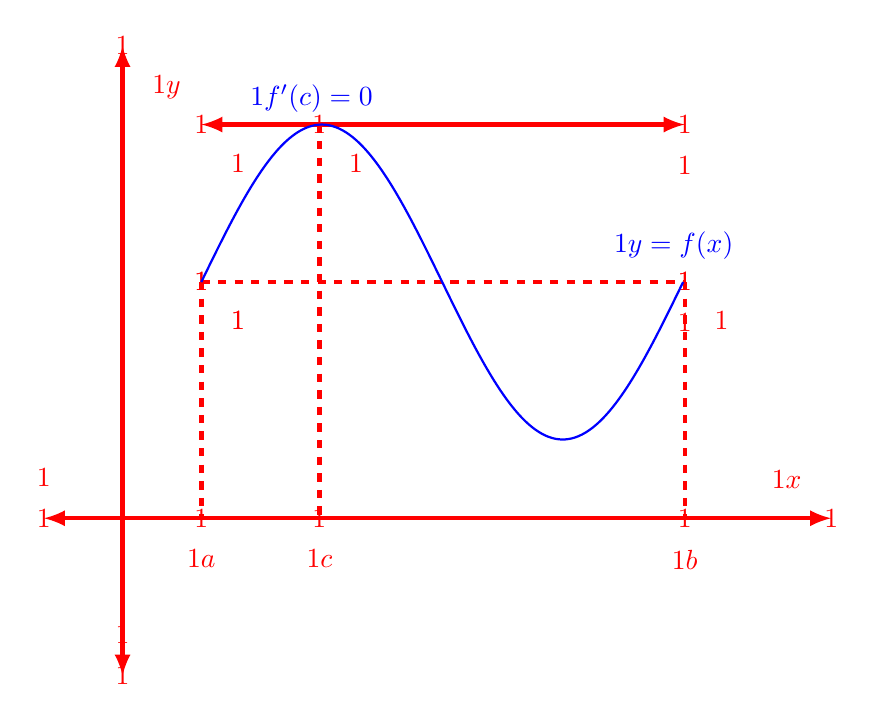
\begin{tikzpicture}[scale=2,
fontscale=1,
         dot/.style = {
     fill = blue,
      circle,
      inner sep =2pt,
      minimum size = 4pt
    }
  ]
%%%%%%%%%%%%%%%%%%%%%%%%%%%%%%%%%%%%%%
% \draw [very thin, style=gray!50, step=0.5] (-0.5,-1.5) grid (3.5,1.5);
 %\draw [thin, gray!60] (0,0) grid (9,9);
\coordinate (O) at (0,0);
\coordinate (O1) at (0,-1.5);
\coordinate (Y) at (-0.5,1.5);
\coordinate (X) at (4,-1.5);
\coordinate (X1) at (-1,-1.5);
\coordinate (Y1) at (-0.5,-2.5);
 \coordinate (A) at( 3.07,0);
\coordinate (A1) at( 3.07,-1.5);
 \coordinate (B) at (3.73,2);
\coordinate (B1) at (3.73,2);
\coordinate (P) at (0.75,1);
\coordinate (P1) at (0.75,-1.5);
\coordinate (C) at (0,0);
\coordinate (D) at (3.73,0);
%%%%%%%%%%%%%%ejes
\draw[color=red,ultra thick,latex-latex]           (X)node[label={above left:$x$}
                               ] {} -- (X1) node[
                               label = {above:$$}] {};
\draw[color=red,ultra thick,latex-latex]           (Y)node[,label={below right:$y$}
                               ] {} -- (Y1) node[
                               label = {above:$$}] {};
%%%%%%%%%%%%%%%%%%%%%%%%%%%%
\draw[color=red,ultra thick,dashed]           (O)node[
                               label = {below right:$$}]{}-- (A) node[
                                label = {below:$$}] {};
\draw[color=red,ultra thick,dashed]           (P)node[
                               label = {below right:$$}]{}-- (P1) node[
                                label = {below:$c$}] {};
\draw[color=red,ultra thick,dashed]           (O)node[
                               label = {below right:$$}]{}-- (O1) node[
                                label = {below:$a$}] {};
\draw[color=red,ultra thick,dashed]           (A)node[
                               label = {below right:$$}]{}-- (A1) node[
                                label = {below:$b$}] {};
\draw[color=red,ultra thick,latex-latex]           (0,1)node[
                               label = {below right:$$}]{}-- (3.07,1) node[
                                label = {below:$$}] {};
\draw[color=blue] (0.7,1.03) node[above =-1pt] {$f'(c)=0$};
\draw[color=blue] (3,0.1) node[above =-1pt] {$y=f(x)$};
%%%%%%%%%%%%%%%%%%%%%%%%%%%%%
\draw [blue, thick, x=0.0085cm, y=1cm,
declare function={f(\x) = sin(\x);
}]
plot [ultra thick,domain=0:360, samples=144, smooth] (\x,{f(\x)});
\end{tikzpicture}